\chapter{Desarrollo}
En este capítulo se detalla el proceso de construcción del sistema SIVEH, partiendo desde el marco metodológico de trabajo hasta la implementación técnica y despliegue de la infraestructura.

\section{Metodología}

Para el desarrollo del sistema de gestión para verificentros se adoptó un enfoque basado en metodolo por fases, con el objetivo de facilitar la organización del trabajo, mejorar la comunicación entre los involucrados y permitir una adaptación constante a los requerimientos del sistema. En particular, se empleó Scrum como metodología principal de gestión del proyecto y Extreme Programming como metodología complementaria enfocada en las prácticas de desarrollo de software.

La combinación de estas metodologías permitió estructurar el trabajo en ciclos de desarrollo cortos, facilitando la entrega progresiva de funcionalidades del sistema y la incorporación de mejoras conforme avanzaba el proyecto.

\subsection{Scrum como metodología principal}

Scrum se utilizó como marco de trabajo para organizar y administrar el desarrollo del sistema. Esta metodología permitió dividir el proyecto en diferentes etapas de trabajo llamadas sprints, en las cuales se desarrollaron y evaluaron funcionalidades específicas del sistema.

El uso de Scrum facilitó la planificación de las actividades, la asignación de tareas y el seguimiento del progreso del proyecto. Entre los elementos más importantes aplicados durante el desarrollo se encuentran:

Definición del Product Backlog: elaboración de una lista priorizada de funcionalidades del sistema, incluyendo el registro de usuarios, control de vehículos, gestión de verificaciones y generación de reportes.

Planeación de sprints: organización del trabajo en periodos de desarrollo cortos que permitieron avanzar de manera progresiva en la construcción del sistema.

Seguimiento del progreso: revisión constante de las tareas realizadas para asegurar que cada funcionalidad cumpliera con los requerimientos establecidos.

Entrega incremental: desarrollo gradual de los módulos del sistema, permitiendo validar su funcionamiento antes de continuar con nuevas características.

Gracias a este enfoque, fue posible mantener un control continuo del avance del proyecto y asegurar que el sistema respondiera a las necesidades planteadas desde el inicio.

\section{Fases de desarrollo}

\subsection{Planificación:} 

En esta etapa se define el objetivo del ciclo y se seleccionan las funcionalidades prioritarias del backlog. Aquí se determinan los cambios técnicos necesarios en el esquema de la Base de Datos (PostgreSQL) o en los modelos de la Aplicación Django, asegurando que los requerimientos operativos del Vericentro se traduzcan en tareas de desarrollo específicas y alcanzables.

\subsection{Ejecución y Seguimiento:} 

Es la fase de desarrollo activo donde se implementa la lógica de negocio en Python. Las reuniones permiten monitorear que el código fluya correctamente a través del servidor Gunicorn (WSGI) y que la configuración de Nginx como proxy inverso permita servir los archivos estáticos de forma eficiente. En esta fase se aplican prácticas de XP como la refactorización constante para mantener la calidad del software que llegará al usuario final vía HTTPS.

\subsection{Revisión:} 

Se presenta el incremento funcional terminado a los interesados para su validación. El éxito de la fase se confirma comprobando el flujo completo mostrado en el diagrama de producción: desde el acceso del cliente por internet hasta el almacenamiento persistente en la base de datos. Esta revisión asegura que las nuevas características son operativas y que la infraestructura soporta la carga de trabajo real.
\\
\begin{figure}[H]
    \centering
    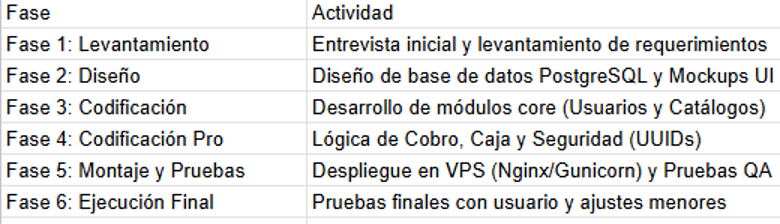
\includegraphics[width=0.8\linewidth]{imagenes/fases.png}
    \caption{Fases de desarrollo}
    \label{fig:fases_desarrollo}
\end{figure}

\section{Arquitectura del Sistema}
Para el desarrollo del sistema se implemento una  arquitectura de tres capas del sistema SIVEH, la cual garantiza una separación clara entre la interfaz, el procesamiento de datos y el almacenamiento. 

\begin{figure}[H]
    \centering
    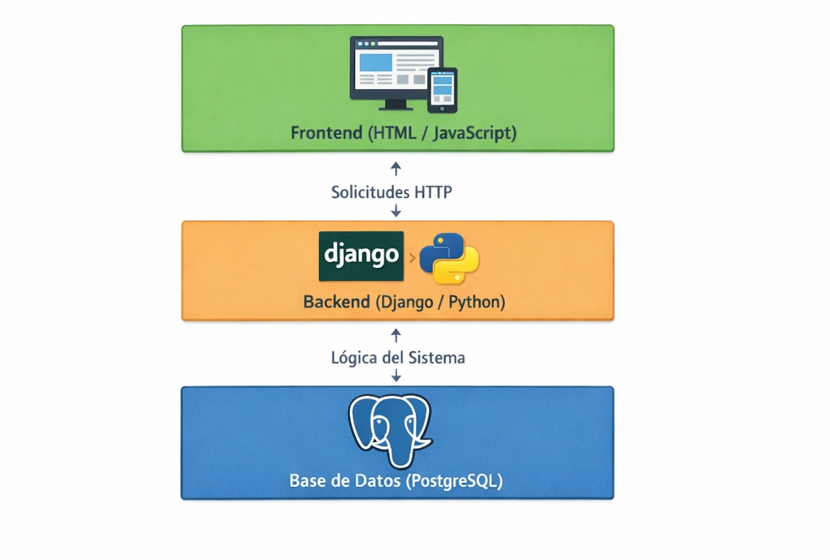
\includegraphics[width=0.8\linewidth]{imagenes/diagrama.png}
    \caption{Diagrama de bloques}
    \label{fig:Diagrama Bloques}
\end{figure}

A continuación, se detalla la función de cada componente y su interacción:

Capa de Presentación (Frontend): Es el entorno con el que interactúa el usuario final, desarrollado en HTML y JavaScript. Su función es capturar los datos de los vehículos y solicitudes administrativas para enviarlos mediante solicitudes HTTP hacia el servidor.

Capa de Lógica de Negocio (Backend): Construida sobre el framework Django y el lenguaje Python, actúa como el núcleo del sistema. Recibe las peticiones del frontend, aplica las reglas de negocio (como la validación de UUIDs o generación de folios) y coordina la comunicación con la base de datos.

Capa de Datos (Base de Datos): Utiliza el motor relacional PostgreSQL para el almacenamiento persistente. Esta capa responde a la lógica del sistema guardando o recuperando información crítica, como registros de verificaciones, inventario de hologramas y reportes financieros, asegurando la integridad y consistencia de toda la operación.

\section{Reingeniería de Procesos}
\begin{figure}[H]
    \centering
    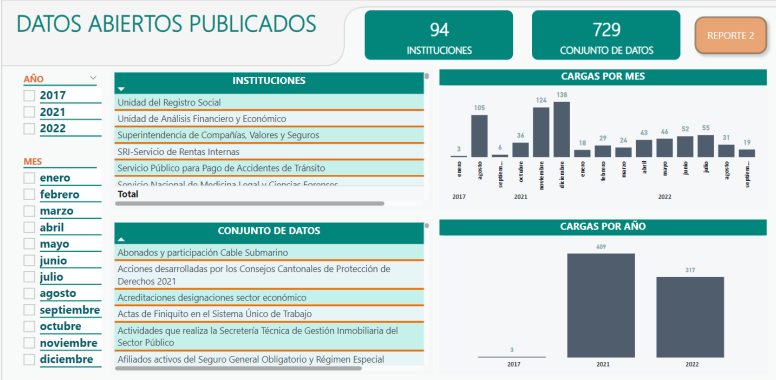
\includegraphics[width=0.8\linewidth]{imagenes/anexo2.png}
    \caption{Diagrama flujo de trabajo SIVEH}
    \label{fig:Flujo SIVEH}
\end{figure}
En la figura \ref{fig:Flujo SIVEH} se presenta la reingeniería del proceso bajo el ecosistema SIVEH. A diferencia del modelo tradicional, la arquitectura permite que la información sea capturada una sola vez y persista a lo largo de todos los módulos. Esta integración asegura que el módulo de caja y el de entrega de resultados consulten la misma instancia de la base de datos PostgreSQL, garantizando la consistencia de los datos y reduciendo el tiempo de atención al usuario final.

\section{Infraestructura de producción del sistema}
A continuación, se presenta la descripción técnica de cada componente de la infraestructura de producción del sistema SIVEH, detallando su función específica dentro del flujo de datos:

\begin{figure}[H]
    \centering
    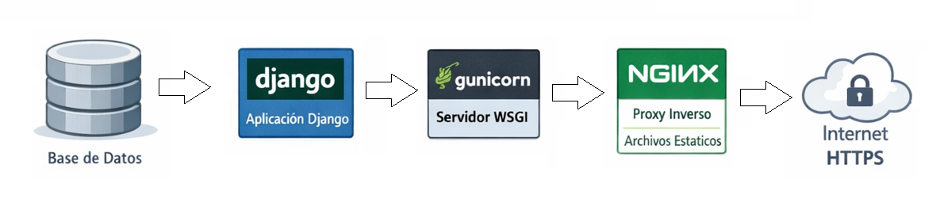
\includegraphics[width=0.8\linewidth]{imagenes/infraestructura.png}
    \caption{Diagrama inf.}
    \label{fig:infraestructura_diagrama}
\end{figure}

\subsection{Base de Datos (PostgreSQL)} 

Es la capa de persistencia donde se almacena toda la información crítica del Vericentro, incluyendo registros vehiculares, inventarios y movimientos financieros. Utiliza PostgreSQL por su robustez y cumplimiento de las propiedades ACID, garantizando que cada transacción sea íntegra y permanente. Esta capa se comunica exclusivamente con la aplicación Django a través del ORM, manteniendo los datos protegidos del acceso externo directo. Se muestra acontinuación el Modelo entidad relación de la base de datos. En el anexo se agrega a detalle las tablas que componen la base de datos ver \autoref{anexo:Tablas BD}. 


\subsection{Aplicación Django} 

Representa el cerebro del sistema o la Lógica de Negocio. Desarrollada en Python, esta capa recibe las peticiones del usuario y decide qué acciones tomar: validar un UUID, calcular una cortesía o generar un reporte contable. Django actúa como el orquestador que consulta la base de datos y renderiza la información necesaria, aplicando siempre filtros de seguridad y permisos de usuario antes de entregar cualquier respuesta.

\subsection{Servidor WSGI (Gunicorn)} 

Debido a que los servidores web tradicionales no pueden ejecutar código Python de forma nativa, se implementa Gunicorn como servidor WSGI (Web Server Gateway Interface). Su función es actuar como un puente o traductor de alto rendimiento que recibe las peticiones HTTP procesadas por el proxy y las convierte en señales que la aplicación Django puede entender y ejecutar. Es el componente encargado de gestionar múltiples procesos simultáneos para que el sistema no se ralentice.

\subsection{Proxy Inverso / Archivos Estáticos (Nginx)}

Nginx cumple una doble función vital en la arquitectura:

Proxy Inverso: Actúa como un escudo y receptor de tráfico; recibe las peticiones de internet y las distribuye eficientemente al servidor WSGI, protegiendo la identidad interna del servidor de aplicaciones.

Gestión de Archivos Estáticos: Se encarga de servir directamente los recursos visuales (CSS, JavaScript e imágenes) sin pasar por Django. Esto libera de carga al backend y acelera significativamente la velocidad de carga de la interfaz de usuario.

\subsection{Internet HTTPS}

Representa el punto de contacto con el usuario final. Toda la comunicación entre el navegador del cliente y el servidor se realiza a través del protocolo HTTPS, lo que significa que los datos viajan cifrados mediante certificados SSL/TLS. Esto garantiza la confidencialidad de la información sensible (como folios de pago y datos de propietarios) y asegura la identidad del servidor de Hostinger ante cualquier intento de interceptación en la red.\\

\section{Codificación e Implementación}

La implementación del sistema SIVEH se estructuró bajo el patrón arquitectónico Modelo-Vista-Template (MVT) de Django, lo que permitió una separación estricta entre la persistencia de datos, la lógica de control y la interfaz de usuario. La orquestación del sistema se centraliza en el archivo \verb|urls.py| para el enrutamiento de peticiones, mientras que la inteligencia operativa reside en  \verb|views.py|.

En esta etapa de codificación, se priorizó la seguridad y la integridad de los datos mediante el uso de Identificadores Únicos Universales (UUIDs) y validaciones a nivel de servidor que previenen la duplicidad de folios. Asimismo, se integraron bibliotecas especializadas como Openpyxl para automatizar la generación de reportes contables en formato  \verb|.xlsx|, y se implementaron selectores dinámicos en las plantillas HTML para minimizar errores de captura manual.

A continuación, se analizan los fragmentos de código más representativos de la lógica del sistema, detallando el funcionamiento de las vistas que gestionan los procesos críticos del verificentro:

\subsection{Vista: reporte\_ventas\_view (Módulo de Administración)}

Esta sección del código corresponde a una vista desarrollada en el framework Django, cuya finalidad es generar reportes financieros dinámicos dentro del sistema SIVEH.

A nivel de programación, esta vista fue construida utilizando el patrón Modelo-Vista-Template (MVT) propio de Django, donde la vista actúa como intermediaria entre la interfaz del usuario y la base de datos. El flujo inicia cuando el administrador envía una solicitud HTTP (generalmente mediante un formulario con filtros de fecha y tipo de pago). El sistema recibe estos parámetros y ejecuta consultas a través del ORM de Django, evitando el uso directo de SQL.

El código realiza principalmente las siguientes acciones:

\begin{itemize}
    \item Valida que el usuario tenga una sesión activa y permisos administrativos, garantizando la seguridad del sistema. 
    \item Filtra los registros de verificaciones y ventas en función de los parámetros proporcionados. 
    \item Realiza operaciones de agregación (sumatorias) directamente en la base de datos, optimizando el rendimiento. 
    \item Organiza los resultados en estructuras de datos que posteriormente son renderizadas en la interfaz. 
\end{itemize}
Adicionalmente, se implementa una funcionalidad de exportación a Excel, la cual se programó utilizando librerías de Python que permiten generar archivos en formato .xlsx. Esta característica facilita la portabilidad de la información y su uso en procesos contables externos.

En resumen, esta vista fue diseñada para automatizar el análisis financiero del verificentro, reduciendo errores humanos y tiempos de procesamiento.\\
\begin{figure}[H]
    \centering
    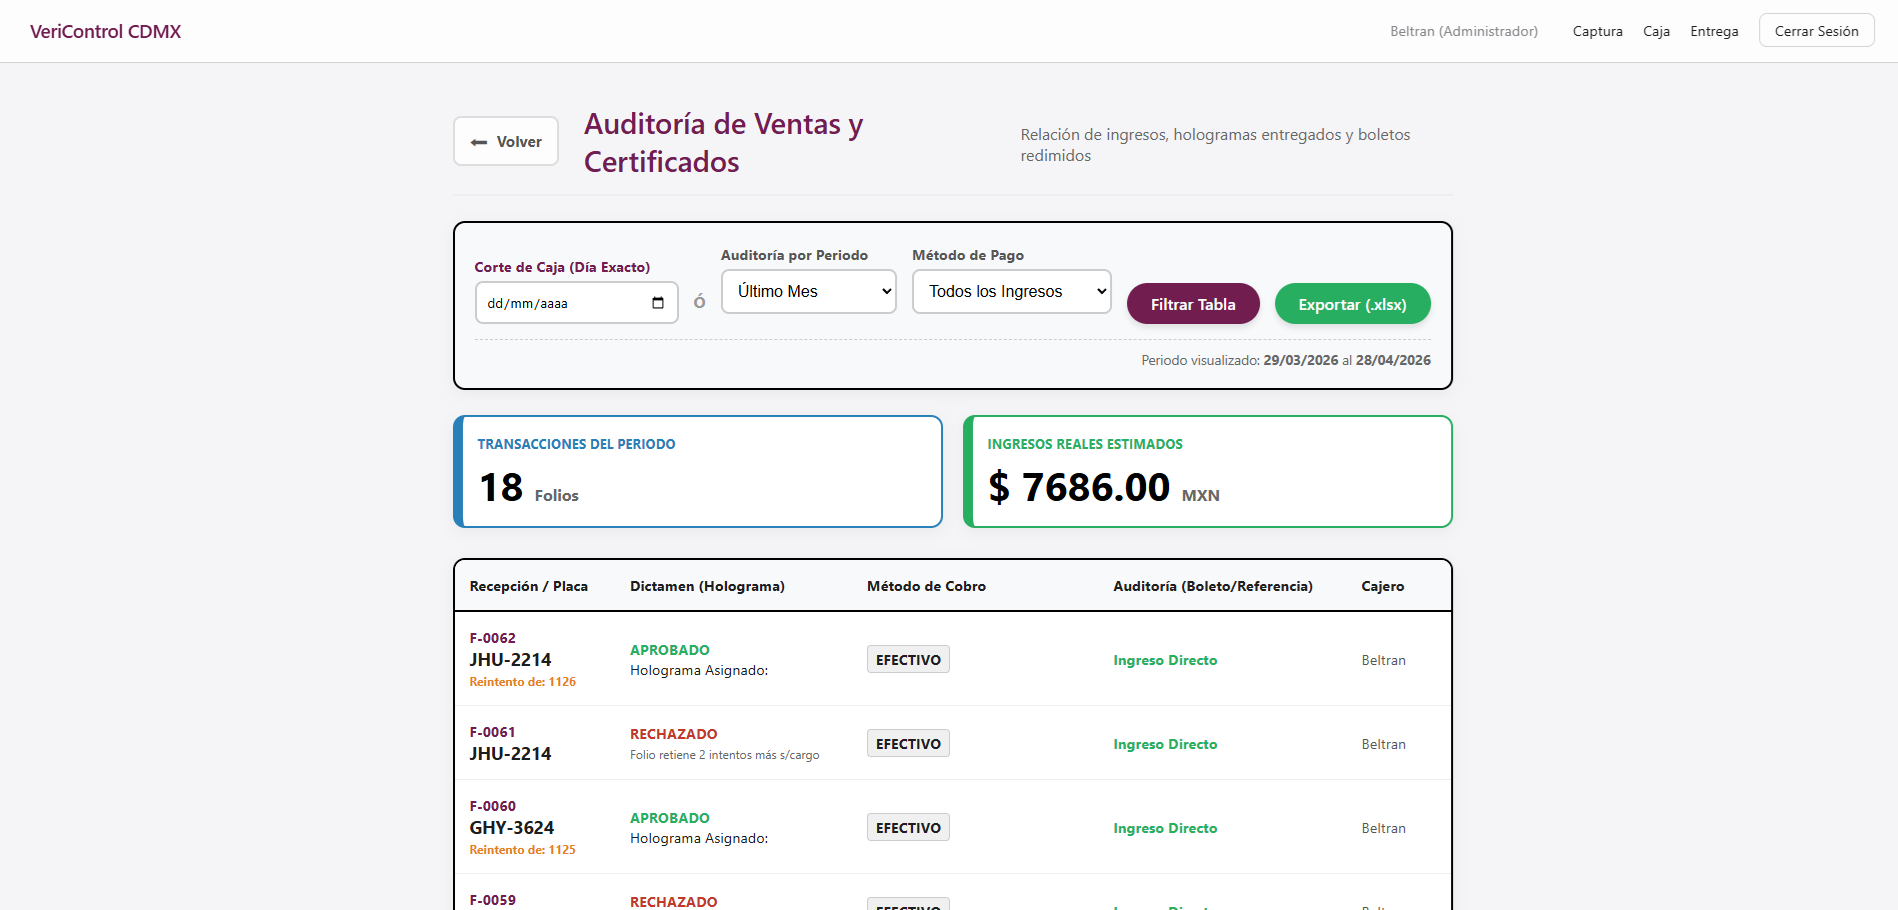
\includegraphics[width=0.8\linewidth]{imagenes/Reporte de ventas.png}
    \caption{Captura }
    \label{fig:Reporte Ven V}
\end{figure}
\begin{figure}[H]
    \centering
    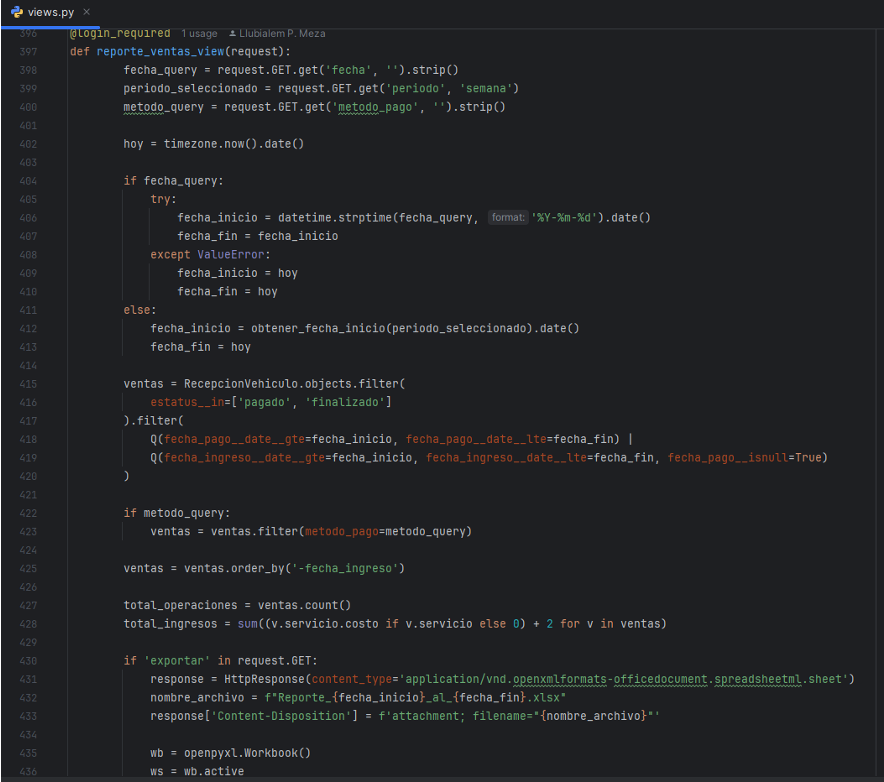
\includegraphics[width=0.8\linewidth]{imagenes/desarrollo1.1.png}
    \caption{Reporte Ventas View}
    \label{fig:reporte_ventas_view}
\end{figure}

\subsection{Vista: captura\_view (Módulo de Recepción)}

Esta vista representa uno de los componentes más críticos del sistema, ya que es responsable del registro y validación de los vehículos que ingresan al proceso de verificación.

Desde el punto de vista técnico, el código fue desarrollado bajo principios de Programación Orientada a Objetos (POO), donde cada entidad (vehículo, taller, servicio) se modela como un objeto dentro del sistema. La vista interactúa con estos modelos mediante el ORM de Django.

El funcionamiento del código se basa en:

\begin{itemize}
    \item Recepción de datos desde formularios en el frontend. 
    \item Validación de campos obligatorios como placas, número de serie y tipo de servicio. 
    \item Verificación de reglas de negocio, como: 
    \begin{itemize}
        \item Evitar registros duplicados en el mismo periodo. 
        \item Validar si el vehículo tiene rechazos previos. 
        \item Determinar si aplica una justificación (multa o reemplazo). 
    \end{itemize}
\end{itemize}
El sistema también implementa restricciones que impiden guardar información incompleta o inconsistente, lo cual se logra mediante validaciones tanto en el frontend (JavaScript) como en el backend (Python).

Otro aspecto importante es el control de permisos, donde solo usuarios autorizados pueden modificar registros existentes. Esto se implementa mediante decoradores de Django y validaciones de sesión.

En términos de desarrollo, esta vista fue programada con enfoque en la integridad de datos, asegurando que toda la información capturada cumpla con las reglas operativas del verificentro antes de almacenarse en la base de datos.
\\
\begin{figure}[H]
    \centering
    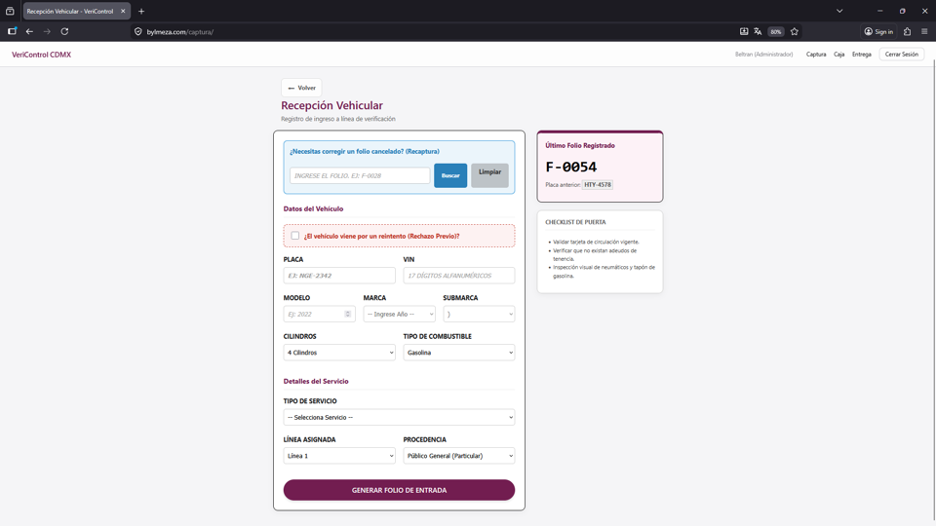
\includegraphics[width=0.8\linewidth]{imagenes/pruebas2.png}
    \caption{Captura }
    \label{fig:Captura V}
\end{figure}

\begin{figure}[H]
    \centering
    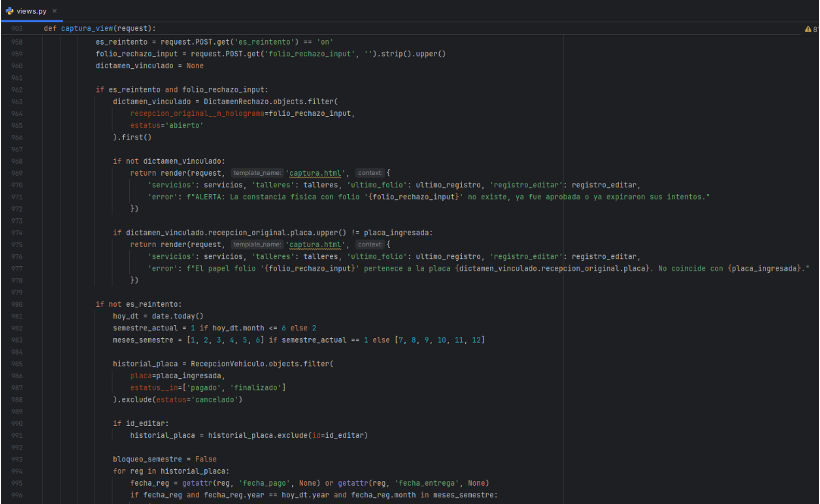
\includegraphics[width=0.8\linewidth]{imagenes/desarrollo1.3.png}
    \caption{Vista Captura-view}
    \label{fig:captura_view_1_3}
\end{figure}

\begin{figure}[H]
    \centering
    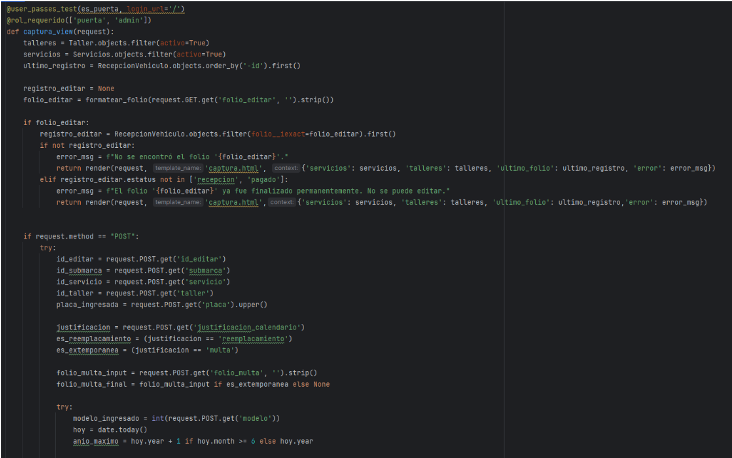
\includegraphics[width=0.8\linewidth]{imagenes/desarrollo1.2.png}
    \caption{Vista Captura-view 2}
    \label{fig:captura_view_1_2}
\end{figure}


\subsection{Vista: caja\_view (Módulo de Cobro)}

El código de esta vista gestiona todo el flujo de pagos dentro del sistema, integrando múltiples métodos de cobro y validaciones comerciales.

A nivel técnico, esta vista se encarga de procesar transacciones, por lo que fue diseñada considerando principios de atomicidad (propiedad ACID de la base de datos). Esto significa que cada operación de pago se ejecuta completamente o no se ejecuta, evitando inconsistencias.

El proceso programado en el código incluye:

\begin{itemize}
    \item Recepción del folio del vehículo previamente registrado. 
    \item Validación de métodos de pago (efectivo, tarjeta, crédito, prepago o cortesía). 
    \item Verificación de boletos de prepago mediante consultas a la base de datos. 
    \item Validación de correspondencia entre el boleto y el taller, evitando fraudes o errores administrativos. 
\end{itemize}
Una funcionalidad destacada es el programa de lealtad, el cual fue implementado mediante lógica condicional en el backend. El sistema lleva un conteo automático de servicios realizados por cliente y, al alcanzar un umbral (ocho servicios), genera un boleto de cortesía.

Finalmente, el código registra:

\begin{itemize}
    \item El usuario (cajero) que realizó la operación. 
    \item El método de pago utilizado. 
    \item La transacción en la base de datos. 
\end{itemize}
Posteriormente, redirige al módulo de impresión de tickets.

Esta vista fue programada para garantizar rapidez en la atención al cliente y precisión en el control financiero.
\\
\begin{figure}[H]
    \centering
    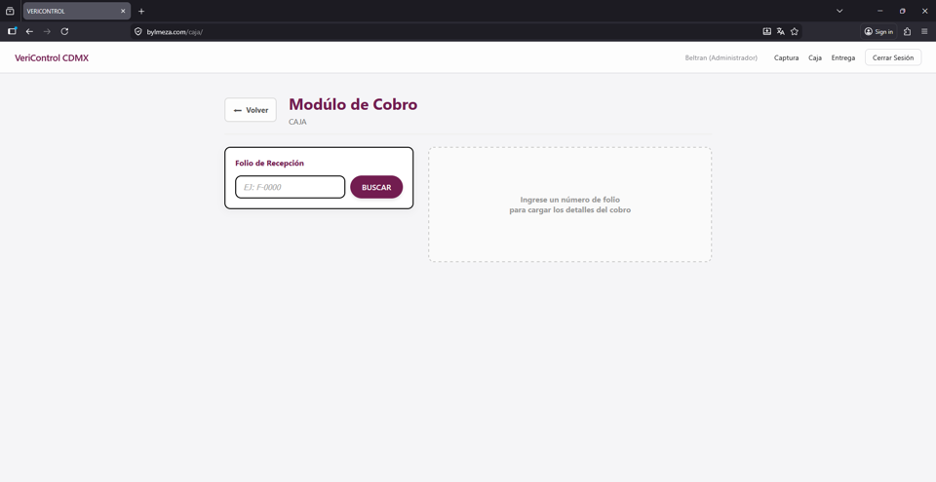
\includegraphics[width=0.8\linewidth]{imagenes/prueba5.png}
    \caption{Caja modulo cobro de servicio }
    \label{fig:caja_modulo_cobro}
\end{figure}

\begin{figure}[H]
    \centering
    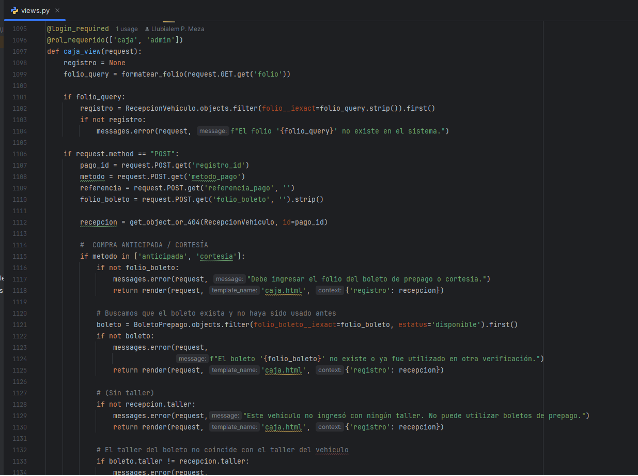
\includegraphics[width=0.8\linewidth]{imagenes/desarrollo1.4.png}
    \caption{Vista caja-view}
    \label{fig:caja_view_1_4}
\end{figure}

\begin{figure}[H]
    \centering
    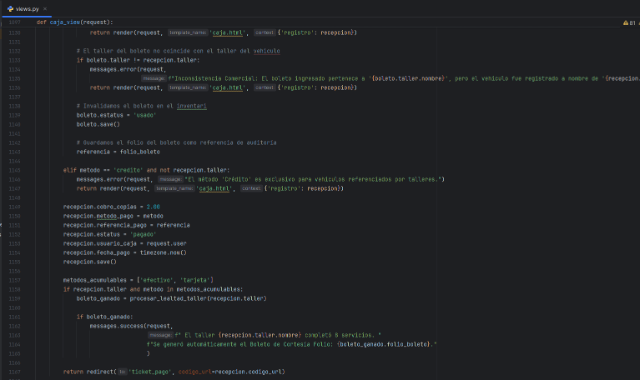
\includegraphics[width=0.8\linewidth]{imagenes/desarrollo1.5.png}
    \caption{Vista caja-view pt.2}
    \label{fig:caja_view_1_5}
\end{figure}


\subsection{Vista: entrega\_view (Módulo de Entrega de Resultados)}

Esta vista corresponde a la etapa final del proceso de verificación vehicular, donde se entrega el resultado y el holograma correspondiente.

El código implementa una lógica automatizada que determina el tipo de holograma basado en características del vehículo, como:

\begin{itemize}
    \item Año modelo 
    \item Tipo de combustible 
    \item Resultado de la verificación (aprobado o rechazado) 
\end{itemize}
A nivel técnico, el flujo del sistema es el siguiente:

\begin{itemize}
    \item Validación de que el pago haya sido realizado previamente (integración con módulo de caja). 
    \item Consulta del inventario de hologramas disponible en la base de datos. 
    \item Asignación automática del siguiente folio físico disponible. 
    \item Registro del dictamen técnico y del usuario responsable. 
\end{itemize}
El sistema también incluye controles de seguridad avanzados:

\begin{itemize}
    \item Restricción de cancelación de hologramas a usuarios con rol administrativo. 
    \item Protección de registros históricos para evitar alteraciones indebidas. 
    \item Trazabilidad completa de cada holograma asignado. 
\end{itemize}
La programación de esta vista se realizó priorizando la sincronización entre módulos y la reducción de errores humanos, utilizando consultas eficientes y validaciones en tiempo real.
\\
\begin{figure}[H]
    \centering
    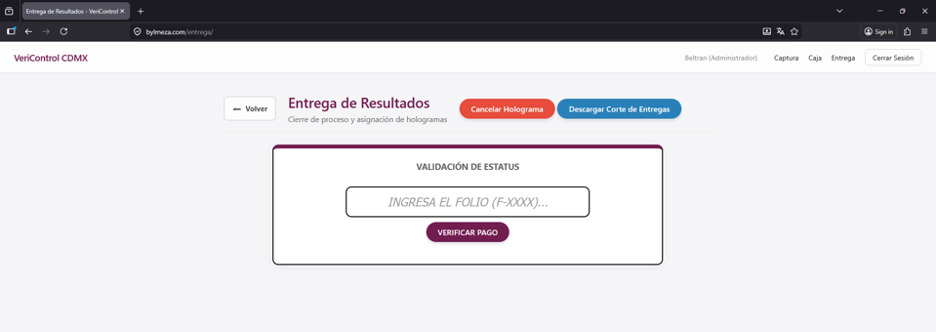
\includegraphics[width=0.8\linewidth]{imagenes/prueba11.png}
    \caption{Entrega de resultados}
    \label{fig:entrega_resultados}
\end{figure}

\begin{figure}[H]
    \centering
    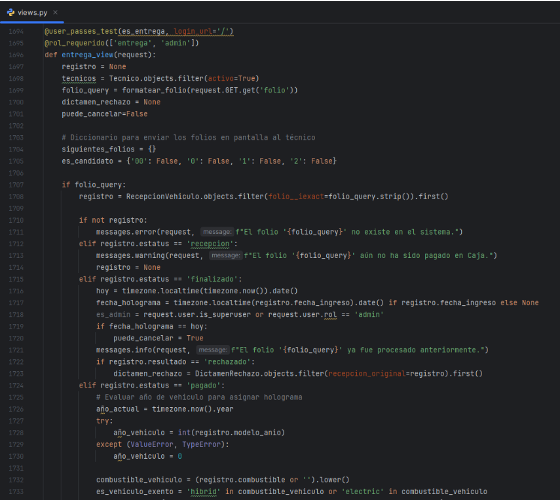
\includegraphics[width=0.8\linewidth]{imagenes/desarrollo1.6.png}
    \caption{Vista entrega view}
    \label{fig:entrega_view_1_6}
\end{figure}

\begin{figure}[H]
    \centering
    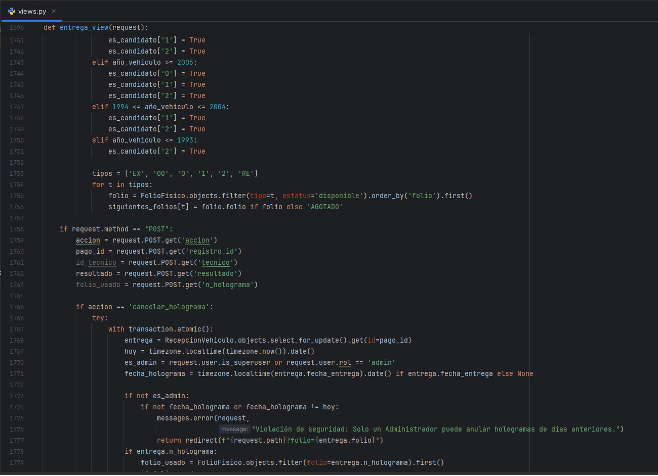
\includegraphics[width=0.8\linewidth]{imagenes/desarrollo1.7.png}
    \caption{Vista entrega view}
    \label{fig:entrega_view_1_7}
\end{figure}


\textbf{Debido a la extensión del proyecto, en este apartado se exponen solo los componentes clave del código. La versión íntegra y funcional del software está disponible para su consulta en el repositorio de GitHub referenciado en el \ref{anexo:github}}
\\

\section{Pruebas}
El objetivo de esta seccion es documentar el proceso de verificación y validación del sistema SIVEH, asegurando que cada componente cumpla con los requisitos técnicos y operativos establecidos. Se aplicó una estrategia de pruebas multinivel para garantizar la estabilidad, seguridad e integridad de los datos en el entorno de producción.
\subsection{Pruebas Unitarias}
Las pruebas unitarias se enfocaron en la verificación de funciones y métodos individuales de forma aislada. En el ecosistema Django, se utilizaron las herramientas nativas de \verb|django.test| para validar la lógica crítica sin depender de factores externos.

\begin{itemize}
    \item \textbf{Validación de UUIDs:} Se comprobó que cada registro generado contara con un identificador único y que el sistema rechazara cualquier intento de acceso mediante ID secuenciales.
    \begin{figure}[H]
    \centering
    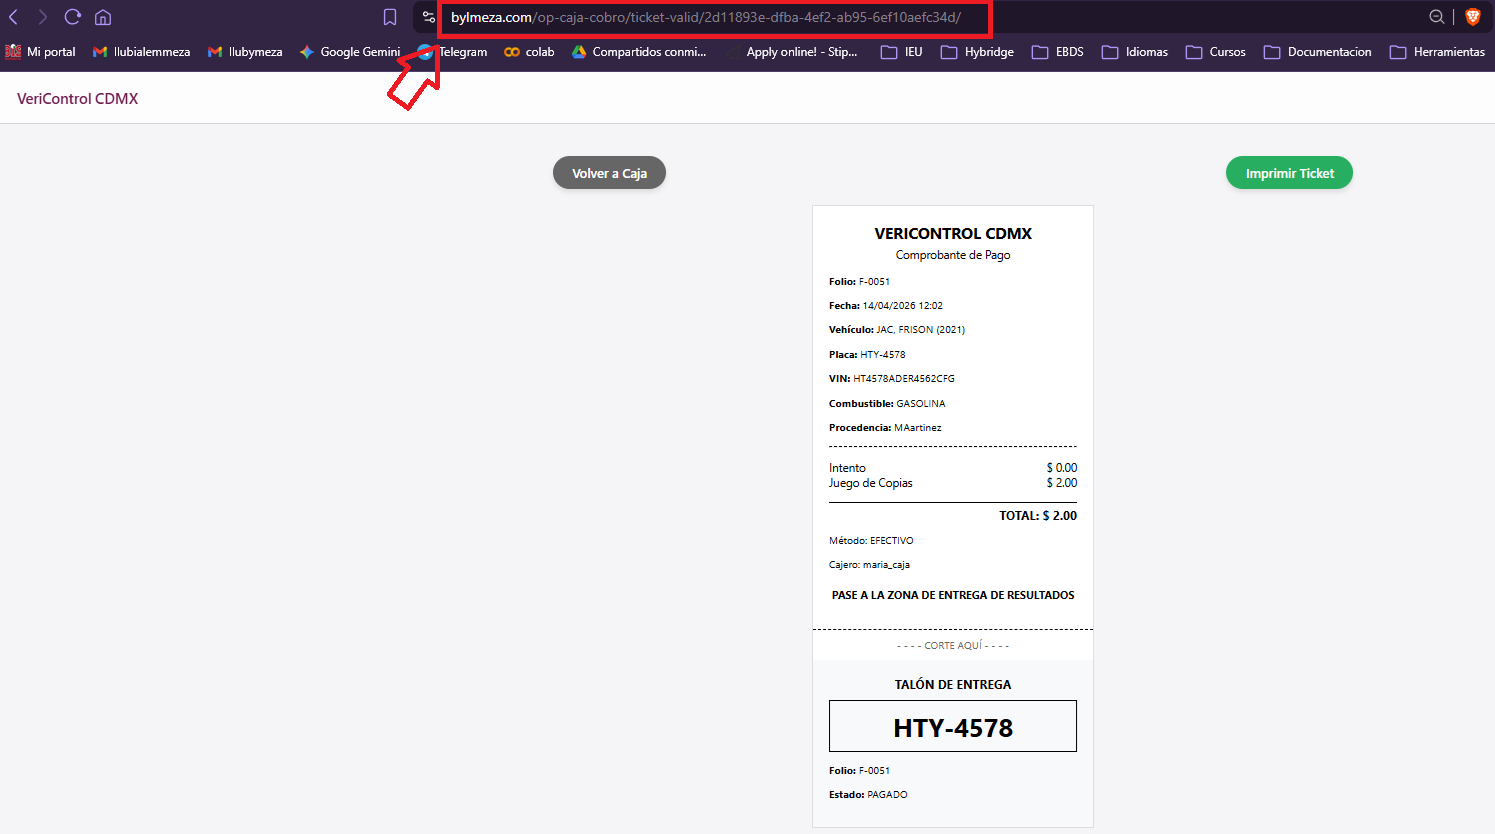
\includegraphics[width=0.8\linewidth]{imagenes/validacion UUID.png}
    \caption{Validacion de UUIDs}
    \label{fig:validacio uuid}
\end{figure}
\begin{figure}[H]
    \centering
    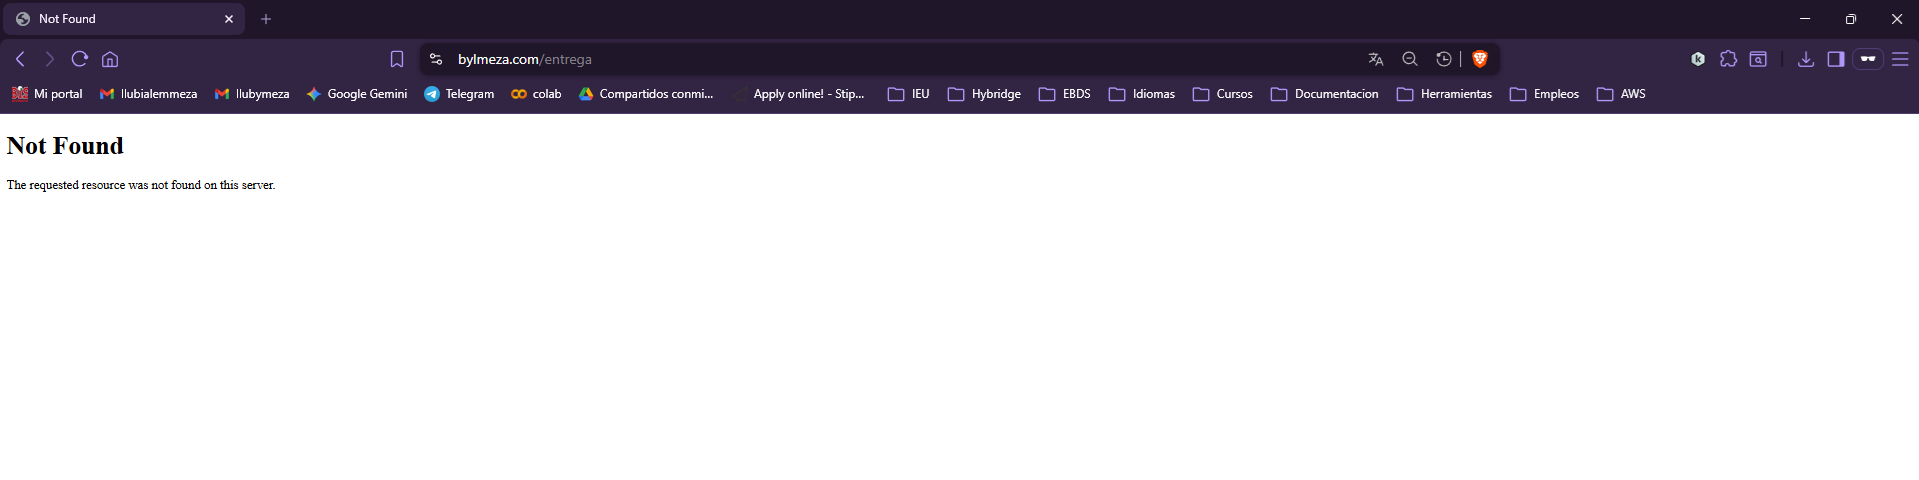
\includegraphics[width=0.8\linewidth]{imagenes/validacion UUID2.png}
    \caption{Intento con ID simple}
    \label{fig:validacion uidd2}
\end{figure}
Las Figuras \ref{fig:validacio uuid} y \ref{fig:validacion uidd2} evidencian la implementación de UUIDs; el sistema rechaza peticiones mediante identificadores secuenciales, protegiendo la información de intentos de enumeración de recursos.

    \item \textbf{Cálculo de Costos y Cortesías:} Se ejecutaron casos de prueba para asegurar que la lógica de 'octava verificación gratuita' se active exactamente al cumplir los criterios, evitando errores en el saldo del cajero.
    \item \textbf{Reglas de Negocio en Modelos:} Se validaron las restricciones de los campos en PostgreSQL, como la imposibilidad de registrar una placa duplicada en el mismo periodo semestral.
\end{itemize}

\subsection{Pruebas de Integración}
Estas pruebas evaluaron la comunicación efectiva entre los diferentes módulos del sistema y las capas de la arquitectura. Se puso especial énfasis en el flujo de datos desde la interfaz hasta la persistencia final.

\begin{itemize}
    \item \textbf{Interacción ORM-Base de Datos:} Se verificó que las consultas complejas realizadas mediante el ORM de Django se tradujeran en transacciones SQL eficientes en PostgreSQL, manteniendo la integridad referencial.
    \item \textbf{Comunicación WSGI:} Se realizaron pruebas de comunicación entre Gunicorn y la aplicación Django para asegurar que las peticiones HTTP fueran procesadas y respondidas sin pérdida de cabeceras de seguridad.
    \item \textbf{Gestión de Archivos Estáticos:} Se validó que Nginx sirviera correctamente los recursos CSS y JavaScript, permitiendo que la lógica del frontend (selectores en cascada) operara en sincronía con los datos del backend.
\end{itemize}

\subsection{Pruebas Funcionales}
Las pruebas funcionales validaron que el sistema respondiera correctamente a las necesidades del usuario final mediante la simulación de escenarios reales.

\begin{itemize}
    \item \textbf{Ciclo Completo de Verificación:} Se simuló el flujo desde la captura inicial del vehículo, el paso por el módulo de caja para el cobro del servicio, hasta la asignación final del holograma.
    \item \textbf{Generación de Reportes:} Se verificó que el módulo de administración generara archivos Excel (.xlsx) con datos precisos, filtrando correctamente por fechas y estados de pago, tal como se especificó en los requerimientos.
    \begin{figure}[H]
    \centering
    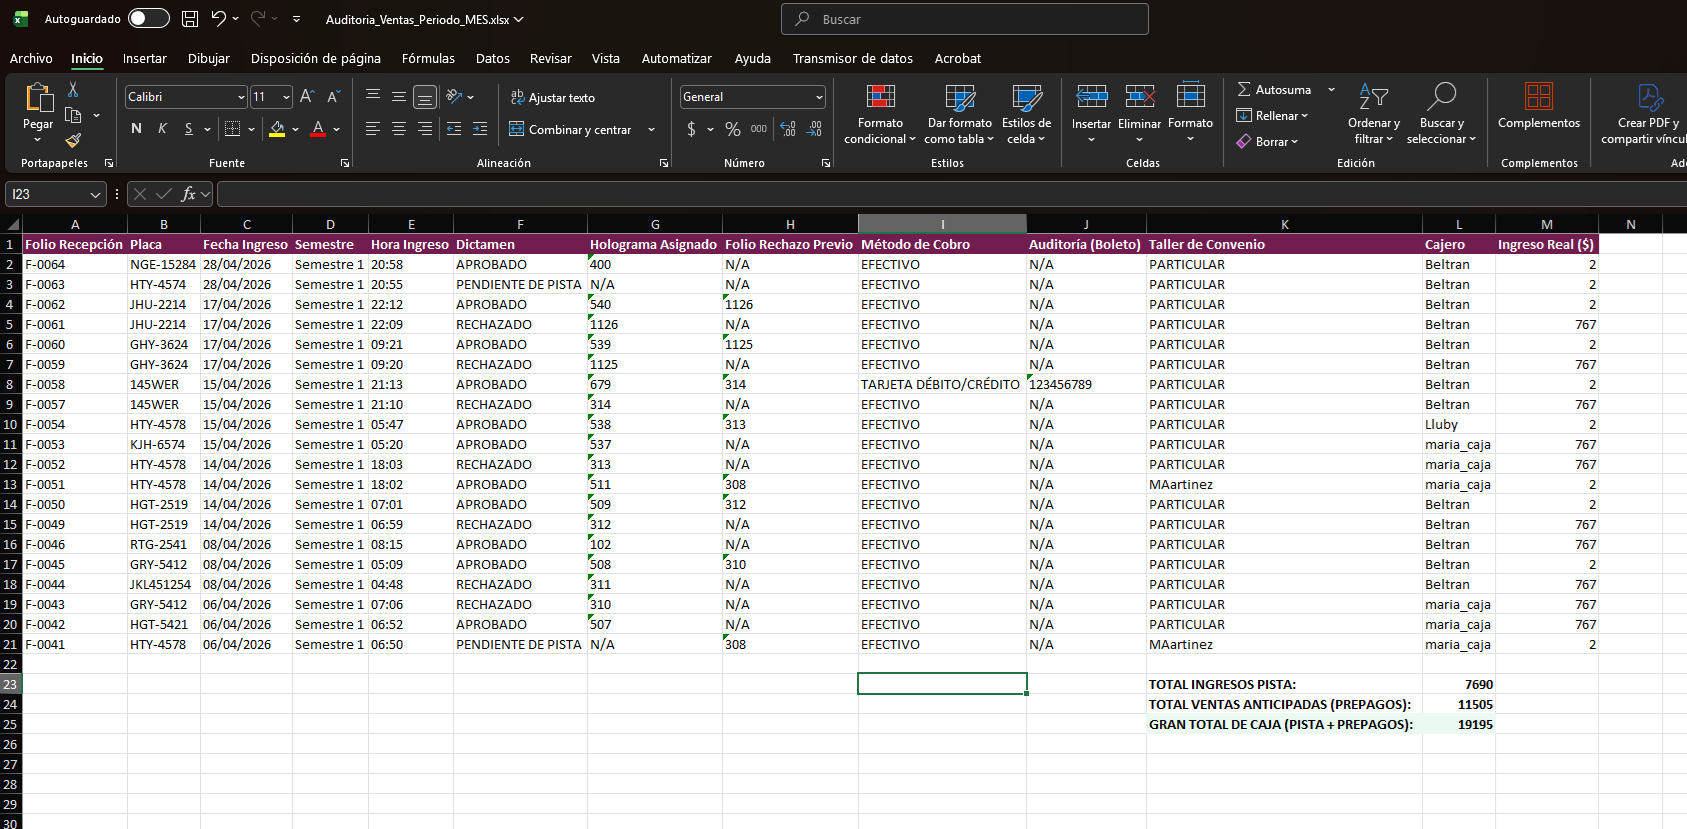
\includegraphics[width=0.8\linewidth]{imagenes/ReporteExcel.png}
    \caption{Reporte generado del ultimo mes}
    \label{fig:Reporte Excel}
\end{figure}
En la Fig.Fig.\ref{fig:Reporte Excel} se muestra el reporte generado por el sistema en formato .xlsx, validando que la integración con la biblioteca Openpyxl extrae correctamente los montos y fechas de la base de datos PostgreSQL.
\end{itemize}

\subsection{Pruebas de Rendimiento}
Dada la naturaleza crítica del tiempo de atención en un verificentro, se midió la respuesta del sistema bajo condiciones de carga en el servidor de producción.

\begin{itemize}
    \item \textbf{Concurrencia:} Se monitoreó el comportamiento del servidor ante múltiples peticiones simultáneas en los módulos de captura y caja, observando que el uso de memoria se mantuvo estable gracias a la gestión de procesos de Gunicorn.
    
\begin{figure}[H]
    \centering
    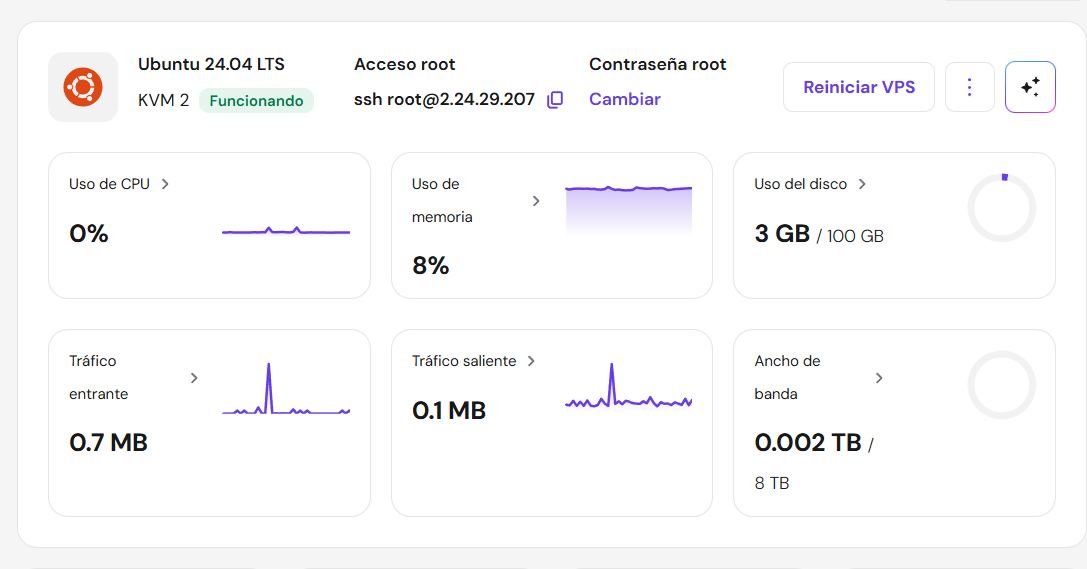
\includegraphics[width=0.8\linewidth]{imagenes/rendimiento.png}
    \caption{Rendimiento VPS}
    \label{fig:Rendimiento}
\end{figure}

    \item \textbf{Tiempos de Respuesta:} Se registraron tiempos de respuesta promedio inferiores a 200ms en consultas locales y menos de 1s en la generación de reportes complejos, cumpliendo con los estándares de eficiencia esperados para una aplicación web moderna.
\end{itemize}



\subsection{Pruebas de Usuario}
Finalmente, el sistema fue evaluado por el personal operativo del verificentro. Estas pruebas se integraron de manera incremental durante las revisiones de los martes, de acuerdo con la metodología Scrum.

\begin{itemize}
    \item \textbf{Usabilidad:} Los usuarios confirmaron que la interfaz reduce la fatiga visual durante jornadas largas de trabajo.
    \item \textbf{Experiencia de Usuario:} Se validó que la reducción de pasos manuales y la eliminación de hojas de cálculo externas facilitan el aprendizaje del sistema para nuevos empleados.
    \item \textbf{Aceptación Final:} El personal administrativo validó la precisión de los cierres de caja automáticos, otorgando el visto bueno para la transición completa al ecosistema SIVEH.
\end{itemize}

